\documentclass[10pt,twocolumn,letterpaper]{article}
\usepackage{xeCJK} % 中文支持
\usepackage{fontspec} % 字体管理
\setCJKmainfont{SimSun} % 指定中文字体（宋体，可换成系统已有字体）

\usepackage[pagenumbers]{iccv}

\newcommand{\red}[1]{{\color{red}#1}}
\newcommand{\todo}[1]{{\color{red}#1}}
\newcommand{\TODO}[1]{\textbf{\color{red}[TODO: #1]}}

\definecolor{iccvblue}{rgb}{0.21,0.49,0.74}
\usepackage[pagebackref,breaklinks,colorlinks,allcolors=iccvblue]{hyperref}
\usepackage{svg}
\usepackage{makecell}
\usepackage{graphicx}
\usepackage{array}
   \usepackage{booktabs} 
   \usepackage{multirow} 

\def\paperID{10}
\def\confName{ICCV}
\def\confYear{2025}

\title{用于实时四旋翼控制的高效自监督神经解析视觉伺服}

\author{
Sebastian Mocanu\textsuperscript{1} \quad
Sebastian-Ion Nae\textsuperscript{1}\thanks{这些作者对本工作贡献相同。} \quad
Mihai-Eugen Barbu\textsuperscript{1}\footnotemark[1] \quad
Marius Leordeanu\textsuperscript{1, 2, 3} \\
\textsuperscript{1}National University of Science and Technology POLITEHNICA Bucharest, Romania \\
\textsuperscript{2}Institute of Mathematics "Simion Stoilow" of the Romanian Academy, Romania \\
\textsuperscript{3}NORCE Norwegian Research Center, Norway \\
{\footnotesize\ttfamily\ \{sebastian.mocanu, sebastian\_ion.nae.stud.fils, mihai\_eugen.barbu.stud.acs\}@upb.ro, leordeanu@gmail.com} 
}


\begin{document}
\maketitle

\begin{abstract}
本文提出一种用于视觉四旋翼控制的自监督神经解析、低成本模型，其中一个仅有 1.7M 参数的小型学生卷积网络能够自动从一个解析教师模型中学习，该教师模型是改进的基于图像的视觉伺服（IBVS）控制器。我们的 IBVS 系统通过简化经典视觉伺服方程并实现高效稳定的图像特征检测，解决了数值不稳定问题。借助知识蒸馏，学生模型相比教师 IBVS 流水线实现了 $11\times$ 的更快推理速度，同时以显著更低的计算和内存开销获得了相近的控制精度。
我们这种仅依赖视觉的自监督神经解析控制，无需显式几何模型或人工标记即可实现四旋翼的姿态调整与运动。所提出的方法结合了仿真到现实的迁移学习，并在无 GPS 的室内环境中借助小型无人机平台进行了验证。我们的主要贡献包括：(1) 一个能够解决经典方法中固有数值不稳定性的解析 IBVS 教师模型，(2) 一个两阶段分割流水线，将 YOLOv11 与基于 U-Net 的掩码分割器结合，用于稳健地进行车辆前后区域分割，从而正确估计目标朝向，以及 (3) 一个高效的知识蒸馏双路径系统，将几何视觉伺服能力从解析 IBVS 教师迁移到一个紧凑的小型学生神经网络中，使其在适用于机载实时部署的同时优于教师模型。
\end{abstract}

\section{引言}
\label{sec:intro}
四旋翼的应用已经从遥控飞行器扩展到用于航拍、测绘和配送的自主系统，通常依赖 GPS、IMU 以及 9 自由度传感器融合 \cite{arreola2018improvement}。虽然这些传感器在室外环境中效果良好，但由于信号干扰、多径效应和标定不确定性，在室内场景中的性能会明显下降 \cite{tang2024control, rebbapragada2024c2fdrone}。基于视觉的传感器成本更低，并且可以通过直接环境感知和即时视觉反馈来弥补这些局限，从而在无 GPS 环境中支持实时特征提取和自主导航所需的空间感知。

需要四旋翼与目标物体进行空间协同的应用，例如自动化仓库巡检系统 \cite{wawrla2019applications} 和动态电影拍摄 \cite{nageli2017real}，都需要稳健的视觉伺服方法。在仓库维护场景中，四旋翼必须在补偿环境扰动的同时，与基础设施部件保持特定距离 \cite{kouris2018learning} 和观察角度 \cite{wawrla2019applications}。类似地，影视拍摄应用要求系统在主体沿复杂轨迹运动时持续调整姿态，以维持期望的构图 \cite{galvane2017automated}。

视觉伺服利用闭环反馈将期望图像特征与当前测量值进行比较，把特征坐标和几何属性作为直接控制输入，而无需显式进行三维姿态重建 \cite{hutchinson1996tutorial, guenard2008practical}。然而，经典的基于图像的视觉伺服（IBVS）方法常常由于交互矩阵中的奇异性以及大幅相机运动时的条件数问题而出现数值不稳定 \cite{corke1996visual}。尽管目标跟踪和姿态对齐任务通常使用 ArUco \cite{kalaitzakis2021fiducial, mraz2020using, cruz2024performance} 或 AprilTag \cite{olson2011apriltag, zhang2017autonomous, banik2025integrating} 等人工标记，这些标记提供了易于检测且具有预定义几何属性的特征，但这类方法仍然面临计算开销和对标记的依赖，从而限制了其在动态、非结构化室内环境中的部署。

我们的工作提出了一种高效的无标记方法：采用自监督解析 IBVS 教师模型，通过简化经典方程并增强图像特征检测来解决数值不稳定问题，同时结合一个轻量级学生神经网络，以实现更优的实时性能。所提出的自监督教师方法集成了两阶段神经网络流程：首先使用 YOLO \cite{redmon2016you, riftiarrasyid2024suitability, yang2025comparative} 实例分割网络进行目标检测，然后在第二阶段将生成的掩码一分为二，以估计玩具车目标的朝向（前后分割），从而在无需人工标记的情况下实现精确的无人机定位。该知识蒸馏框架将改进 IBVS 教师的解析稳定性迁移到一个更高效、低成本的学生网络中，同时获得更好的控制性能。系统验证采用渐进式方法，先进行基于仿真的训练，再引入真实世界数据进行微调。

实验设置所需的硬件基础设施极为简单，仅包括一台标准笔记本电脑和与四旋翼平台的无线通信链路，这表明该方法在室内自主运行中具有实际可行性，同时也面向未来的边缘端部署。

\section{基于视觉的伺服}
\label{sec:related_work}
视觉伺服是移动机器人中一种基于相机反馈的基础控制范式。经典方法可分为基于位置的视觉伺服（PBVS）和基于图像的视觉伺服（IBVS）。PBVS 从图像特征重建三维姿态，以实现笛卡尔空间控制\cite{qin2023perception, sun2025towards}；而 IBVS 则直接使用图像特征作为反馈信号，从而规避姿态估计中的不确定性\cite{corke1996visual, yang2020autonomous, lee2012adaptive}。对于实时机器人应用，由于其计算效率和鲁棒性，IBVS 更常被采用 \cite{yang2024high, kumar2024tracking}。

IBVS 控制律可表示为：

\begin{equation}
\mathbf{v} = -\lambda \mathbf{L}_s^+ (\mathbf{s} - \mathbf{s}^*)
\end{equation}

其中，$\mathbf{v} = [v_x, v_y, v_z, \omega_x, \omega_y, \omega_z]^T$ 表示相机速度螺旋量（线速度和角速度），$\lambda$ 为控制增益，$\mathbf{s}$ 为当前图像特征，$\mathbf{s}^*$ 为期望特征。

交互矩阵 $\mathbf{L}_s$（图像雅可比矩阵）将特征运动与相机运动关联起来：

\begin{equation}
\dot{\mathbf{s}} = \mathbf{L}_s \mathbf{v}
\end{equation}

对于深度为 $Z$、像素坐标为 $(u, v)$ 的每个点，交互矩阵为：

\begin{equation}
\label{eq:ibvs-full}
\mathbf{L}_s = \begin{pmatrix}
-\frac{f}{Z} & 0 & \frac{\bar{u}}{Z} & \frac{\bar{u} \bar{v}}{f} & -\frac{f^2 + \bar{u}^2}{f} & \bar{v} \\
0 & -\frac{f}{Z} & \frac{\bar{v}}{Z} & \frac{f^2 + \bar{v}^2}{f} & -\frac{\bar{u} \bar{v}}{f} & -\bar{u}
\end{pmatrix}
\end{equation}

其中，$\bar{u} = u - u_0$、$\bar{v} = v - v_0$ 是相对于主点的像素坐标，$f$ 为以像素为单位表示的焦距。

伪逆 $\mathbf{L}_s^+$ 计算如下：

\begin{equation}
\mathbf{L}_s^+ = (\mathbf{L}_s^T \mathbf{L}_s)^{-1} \mathbf{L}_s^T
\end{equation}

特征检测是 IBVS 实现中的关键组成部分。由于其可靠性和实现简单性，基于标记的方法占据主导地位。Inria 展示了使用 Parrot Bebop 2 进行 ArUco 标记跟踪以服务于移动目标应用\cite{Marchand05b}，以及基于 PID 的移动目标跟踪\cite{teuliere2011chasing}。类似的基于标记系统也已被用于自主无人机降落和表面检测任务\cite{keipour2022visual, drones8110605}，证明了其在真实场景中的有效性。
然而，基于标记的方法在实践中存在局限，包括对环境条件的敏感性，例如光照变化、部分遮挡和标记退化。此外，标记的安装与维护需求也限制了其在动态或难以接近环境中的适用性 \cite{liang2020moving}。

深度学习的最新进展带来了替代性的特征检测方法。神经网络作为关键点检测器已被用于特定目标跟踪，正如 \cite{sepahvand2025deep} 所示，其中一个 CNN 被训练用于在不同光照和遮挡条件下检测矩形物体上的关键点。其他工作则关注在激烈机动过程中进行边界框检测和目标中心跟踪 \cite{10140151}。
YOLO 系列模型已被广泛应用于机器人任务 \cite{li2023design, zhang2024vision}，包括实例分割 \cite{mohamed2021insta, tang2024visual}、目标检测 \cite{drones8110605} 和图像分类 \cite{zhao2024real}，这表明深度学习方法在视觉伺服特征提取方面具有很强的通用性 \cite{pathre2024imagine2servo}。

近期方法将神经网络与视觉伺服算法结合，以增强机器人控制。Liu 等人\cite{liu2019image} 开发了一个用于机械臂操作的双流网络，能够直接输出速度指令以实现期望姿态，而无需显式的视觉伺服计算。知识蒸馏技术在轻量级伺服网络中也展现出潜力，正如 \cite{drones8110605} 所示，其中一个学生网络学习了树枝操作中的最优抓取点识别。

我们的工作通过从结合 IBVS 算法的 YOLO 分割网络中蒸馏知识来扩展这些概念，在保持计算效率的同时消除了对人工标记的需求。所提出的轻量网络能够直接从单帧相机图像生成速度指令。此外，我们通过持续学习来缩小仿真到现实之间的差距：先在仿真中训练，再使用真实世界数据进行微调，以确保其在不同部署环境中的稳健表现。

\section{我们的方法}
\label{sec:proposed_method}
\begin{figure*}[t]
    \centering
    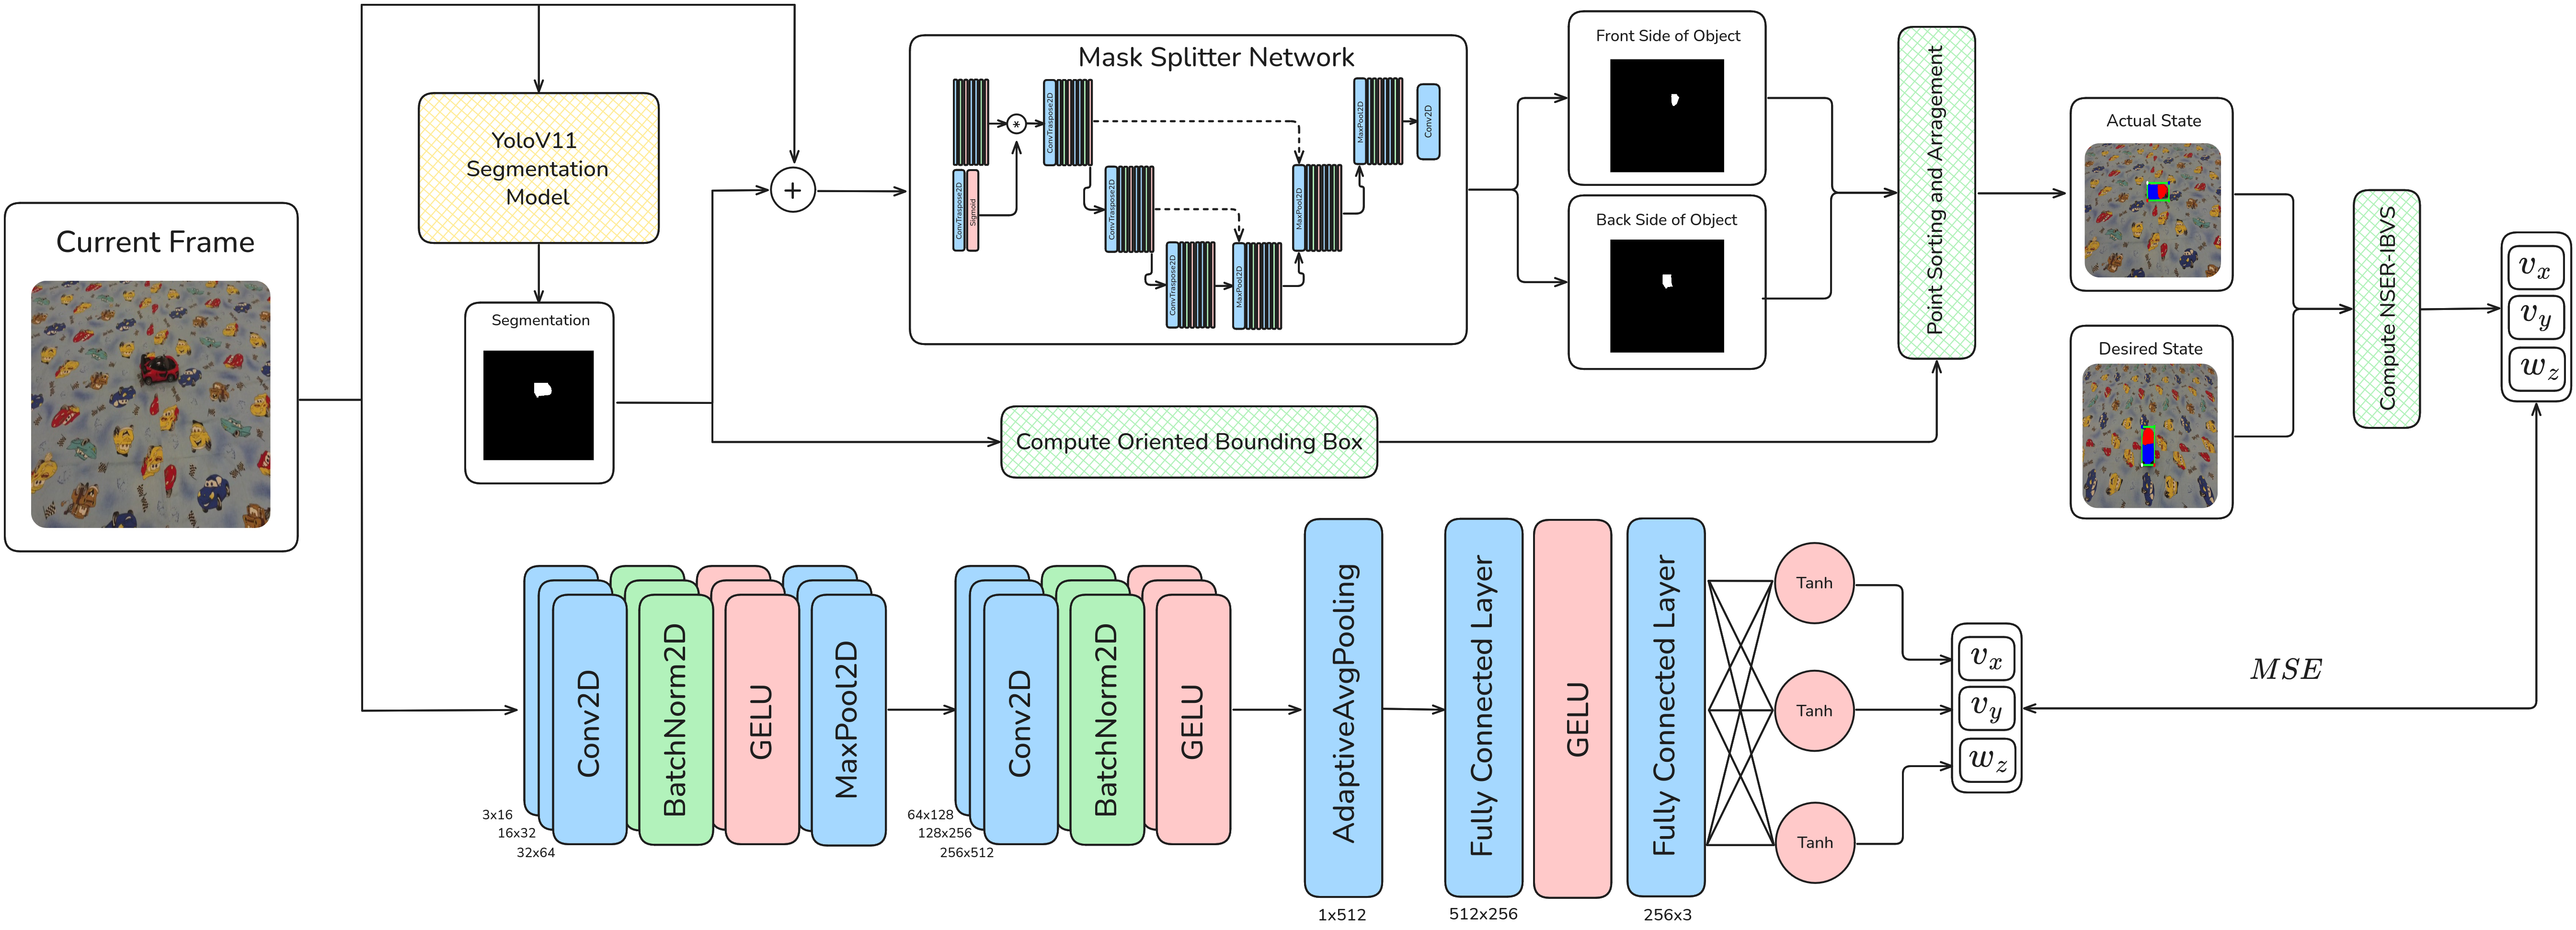
\includegraphics[width=\textwidth]{teacher-student-math.png}
    \caption{所提出的师生式自监督神经解析模型概览。上排展示了 NSER-IBVS（解析）教师路径，该路径使用 YOLO 进行目标分割，并通过掩码分割网络估计物体相对于无人机相机的朝向。下排表示学生路径，其通过最小化自身输出的无人机指令（$\nu_x$、$\nu_y$、$\omega_z$）与教师输出之间的 MSE 损失进行学习。}
    \label{fig:teacher-student-math}
\end{figure*}

我们的方法由一个用于基于视觉的四旋翼控制的师生框架组成，教师和学生都在真实世界环境的数字孪生中进行测试。

教师采用一个与基于图像的视觉伺服算法相结合的两阶段神经网络处理系统。在第一阶段，使用一个小型 YOLOv11 Nano（2.84M 参数）实例分割网络。该网络先在数字孪生生成的合成数据上训练，随后使用真实图像进行微调。这一阶段有两个主要目标：计算车辆的有向边界框（OBB），并将其掩码提供给系统的第二阶段，因为仅靠 OBB 无法实现准确的姿态推断。第二阶段是一个专门设计的神经网络，用于将 YOLO 掩码一分为二，生成代表目标车辆前部和后部区域的掩码。知道前后掩码的位置并结合 OBB 后，我们可以重新排列关键点，生成四个有序点（每个区域两个），作为 IBVS 的稳定视觉特征。随后利用这些特征计算图像雅可比和控制速度，以最小化误差并达到期望的相对状态。期望的朝向关键点通过在开始时捕获目标姿态、进行分割并提取相应特征点来建立。然后，我们对这些关键点进行稳定性预处理，具体细节见第 \ref{sec:ibvs_implem} 节。随后该方法相对于期望参考姿态进行姿态校正。

该框架构成教师模型，并被蒸馏为一个紧凑的卷积神经网络；该网络通过回归学习，从相机输入的 RGB 图像中输出四旋翼控制速度，相关细节见第 \ref{sec:know_dist} 节。


\begin{figure*}[t]
    \centering
    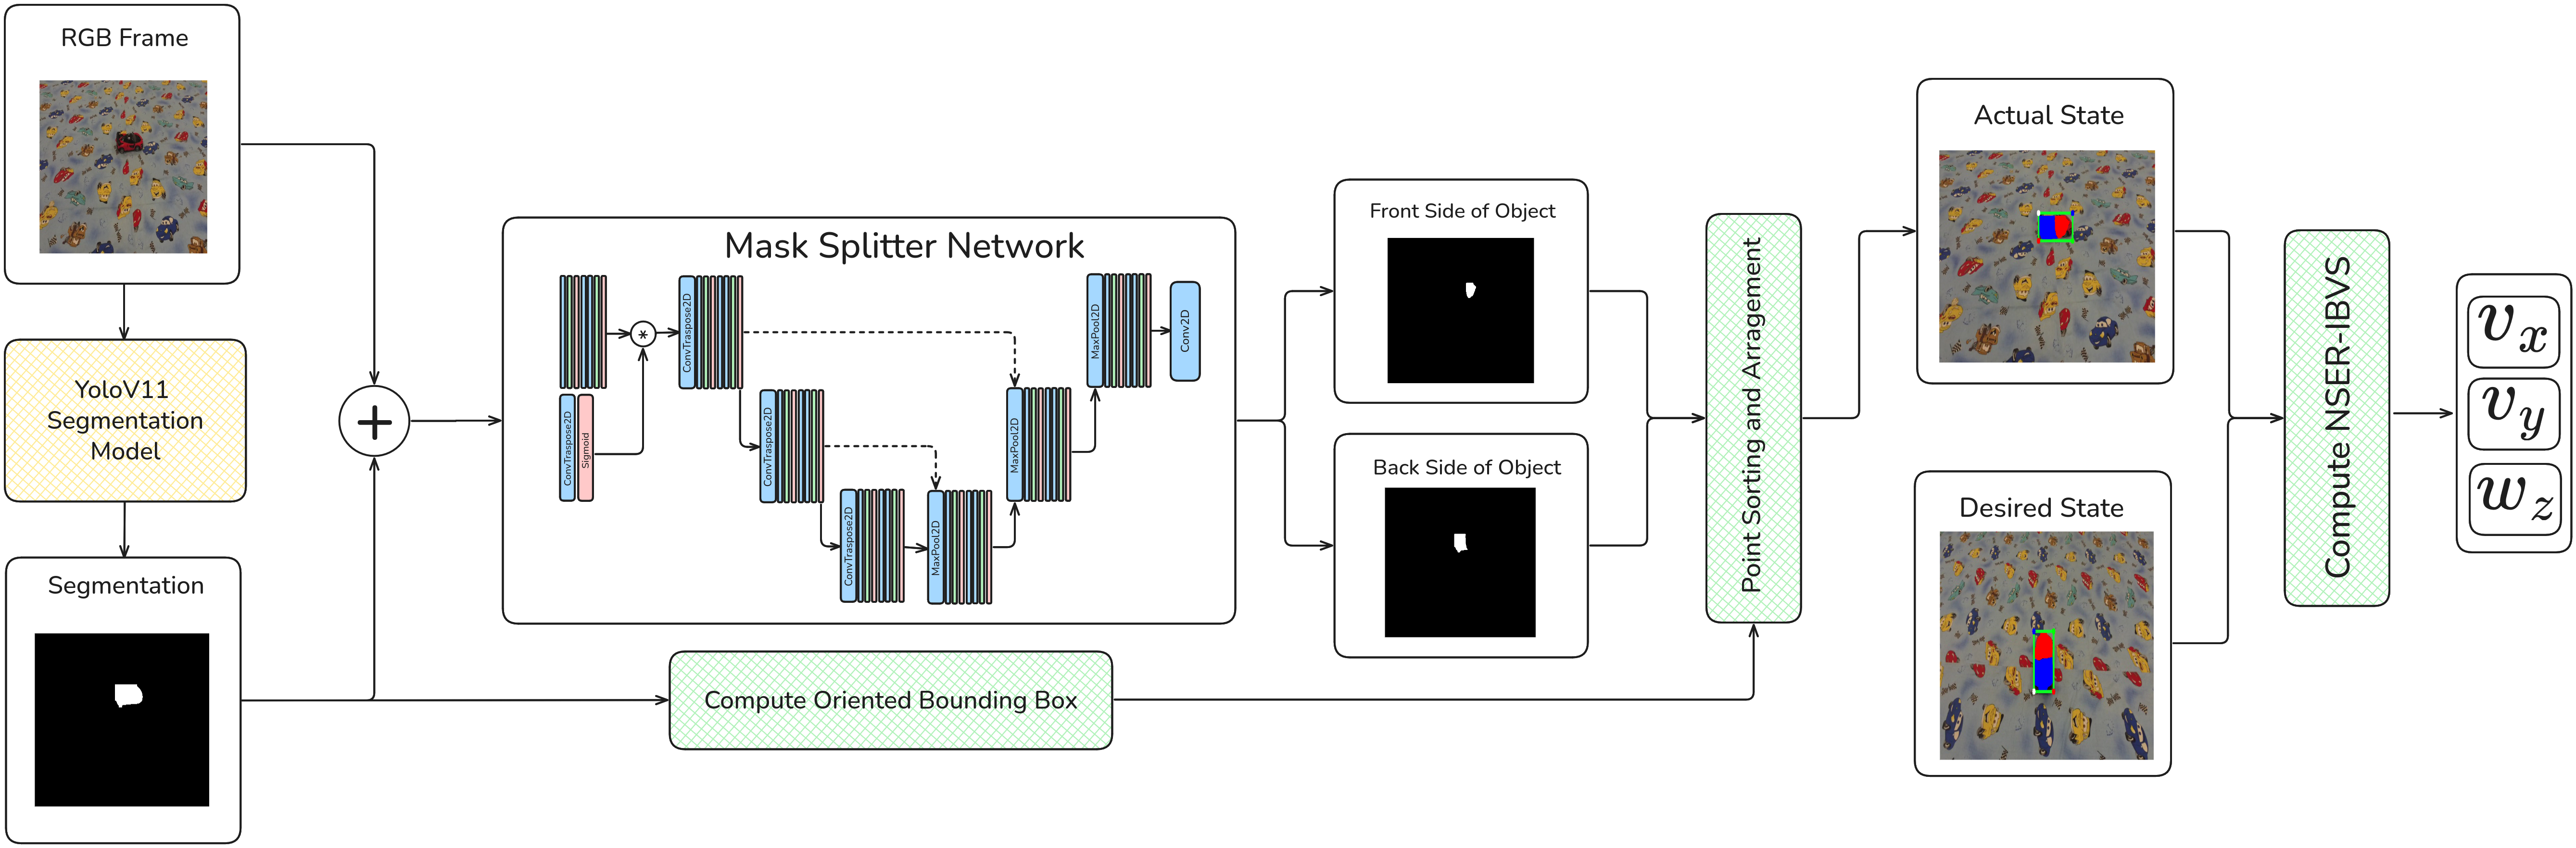
\includegraphics[width=\textwidth]{NSER-IBVS.png}
    \caption{所提出的数值稳定、高效、简化的基于图像视觉伺服（NSER-IBVS）架构概览。该流程接收一帧 RGB 图像，生成分割结果，并将其作为掩码分割网络的输入。从原始分割结果中确定边界框坐标，并将其与分离后的前后掩码结合起来重新排列坐标位置。这些坐标作为解析模型的视觉特征，用于计算速度指令（$\nu_x$、$\nu_y$、$\omega_z$）。}
    \label{fig:nser-ibvs}
\end{figure*}

\subsection{数值稳定的高效简化 IBVS}
\label{sec:ibvs_implem}

所提出的方法首先使用仿真生成的数据训练 YOLOv11 Nano 实例分割模型，作为两阶段分割流水线的基础。第一阶段对整辆车进行分割，而第二个网络将分割区域划分为前部和后部，如图 \ref{fig:nser-ibvs} 所示。虽然第一阶段在分割上有效，但其生成的边界框可能包含不属于目标的部分。为解决这一问题，我们在分割出的目标掩码外计算边界框。这会在推理时产生不稳定的点排序，从而为解析 IBVS 算法带来不一致性。通过确定前后掩码的位置，我们可以重新排列这些点，构造一个更能表示车辆姿态且提供更稳定特征点的有向边界框，如图 \ref{fig:bb-vs-obb-yolo-seg} 所示。

\begin{figure}[!ht]
    \centering
    \begin{minipage}[b]{0.31\linewidth}
        \centering
        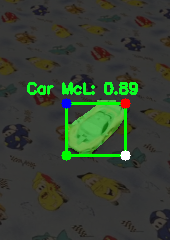
\includegraphics[width=\linewidth]{car-seg-simple.png}
    \end{minipage}
    \hfill
    \begin{minipage}[b]{0.31\linewidth}
        \centering
        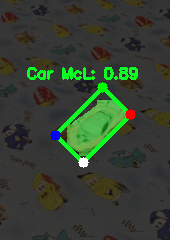
\includegraphics[width=\linewidth]{car-seg-semi-oriented.png}
    \end{minipage}
    \hfill
    \begin{minipage}[b]{0.31\linewidth}
        \centering
        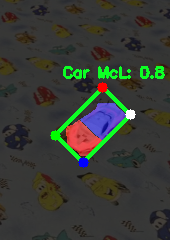
\includegraphics[width=\linewidth]{car-seg-mask-splitter.png}
    \end{minipage}
    \caption{由分割结果得到的不同边界框方法对比：（左）常规边界框，包含不属于目标的部分；（中）在不同帧之间朝向可能变化的有向边界框；（右）利用掩码分割网络分离车辆前后组件以提升排序稳定性的有向边界框。}
    \label{fig:bb-vs-obb-yolo-seg}
\end{figure}


掩码分割网络采用带注意力机制 \cite{oktay2018attentionunetlearninglook} 的 U-Net \cite{ronneberger2015unetconvolutionalnetworksbiomedical} 架构，输入为一个 4 通道张量，包含原始 RGB 图像和来自 YOLOv11 的二值车辆掩码。该编码器-解码器结构带有跳跃连接，并通过三个阶段逐步下采样，通道维度分别为 32、64、128 和 256。应用于掩码通道的注意力机制会生成空间权重，用于调制图像特征，使其聚焦于车辆区域。解码器通过转置卷积重建空间分辨率，输出一个 2 通道结果，分别表示前部和后部分割掩码。该网络约含 1.94M 参数，并在较深层引入 dropout 正则化以防止过拟合。

分割器损失函数通过重建原始输入掩码，将二值分割掩码划分为互补的前后区域。多个约束共同确保正确分割：单独的二元交叉熵损失保证每个预测掩码与其真实标签一致，分割约束在两个预测掩码之和与原始掩码不一致时进行惩罚，而重叠惩罚则抑制同一像素被同时占用。覆盖损失通过对超出原始掩码的多余预测以及掩码内部被遗漏区域进行惩罚来确保准确重建。训练过程中损失权重会动态调整，先强调单个掩码的准确性，再逐步转向更强的分割与重叠约束。

随后对得到的分割掩码进行处理，通过对目标边界拟合最小外接矩形来计算有向边界框。该边界框的四个角点坐标作为 IBVS 框架的视觉特征。为确保关键点稳定性和排序一致性，我们采用了一种预处理算法，根据点到各自掩码质心的距离，将其分配到前部或后部区域。随后将这些点按顺时针顺序排列，以保持跨帧的时序一致性，从而避免可能破坏 IBVS 控制回路的特征对应歧义。

控制速度的计算通过比较当前关键点坐标与从期望姿态配置中获得的参考特征来实现。由于四旋翼平台是欠驱动的，我们采用一种高效方法，只从经典 IBVS 控制器中计算必要的速度分量，即去除角速度分量 $\omega_x$ 和 $\omega_y$ 以及线速度 $\nu_z$。此外，由于我们的控制器仅在固定高度下工作，我们也移除了线速度分量 $v_z$。

Starting from Equation \ref{eq:ibvs-full}, the reduced interaction matrix takes the form:
\begin{equation}
\label{eq:numerical-stable-efficient-reduced-ibvs}
\begin{pmatrix}
\dot{u} \\
\dot{v}
\end{pmatrix} = \begin{pmatrix}
-\frac{f}{Z} & 0 & \bar{v} \\
0 & -\frac{f}{Z} & -\bar{u}
\end{pmatrix} \begin{pmatrix}
v_x \\
v_y \\
\omega_z
\end{pmatrix}
\end{equation}

我们据此堆叠来自有向矩形关键点对应的雅可比矩阵。

\subsection{师生模型蒸馏}
\label{sec:know_dist}

为实现实时部署，我们采用知识蒸馏 \cite{hinton2015distillingknowledgeneuralnetwork}，将视觉伺服能力从教师 IBVS 流水线迁移到一个轻量、低成本的学生网络。该学生网络被设计为一个 1.7M 参数的 CNN，使用均方误差（MSE）损失直接从 RGB 图像回归控制速度。

该架构的一个关键组成部分是对目标标签（速度指令）的归一化，以及在推理时进行相应的反归一化。训练该学生网络需要 RGB 图像及其对应的控制速度。我们分析了在真实世界和数字孪生环境中实验得到的数值，并确定了所有场景下每个指令的最小和最大边界，如表 \ref{tab:cmd-values} 所示。对目标标签进行归一化可通过确保所有速度指令处于相似的数值范围来提升训练稳定性，避免某些输出由于尺度差异而主导损失函数。该方法还能改善反向传播过程中的梯度流，并支持使用如 tanh 之类的有界激活函数，从而在保持整个训练过程可微的同时，自然地将网络输出限制在物理上有意义的控制范围内。

\begin{table}[h!]
    \centering
    \begin{tabular}{lcc|cc|cc}
        & \multicolumn{2}{c}{$\nu_{x}$} & \multicolumn{2}{c}{$\nu_{y}$} & \multicolumn{2}{c}{$\omega_{z}$} \\
        \cmidrule(lr){2-3} \cmidrule(lr){4-5} \cmidrule(lr){6-7}
        & min & max & min & max & min & max \\
        \hline
        仿真  & -24 & 16 & -9 & 9 & -27 & 40 \\
        真实 & -30 & 30 & -30 & 30 & -40 & 40 \\
        \bottomrule
    \end{tabular}
    \caption{在数字孪生（Sim）和真实世界（Real）环境中，通过 NSER-IBVS 评估运行收集得到的平移速度 $\nu_{x}$、$\nu_{y}$ 以及旋转速度 $\omega_{z}$ 的最小和最大指令值。用于确定自监督方法中目标标签的归一化范围。}
    \label{tab:cmd-values}
\end{table}

学生网络结构由卷积特征提取器和全连接回归层组成。卷积主干通过六个卷积块将通道维度从 16 逐步提升到 512，每个块都包含批归一化和 GELU 激活函数。前两个块之后使用最大池化进行空间下采样，而最后几层使用 3x3 的卷积核以捕获细粒度空间特征。自适应全局平均池化层将空间维度压缩到 1x1，随后接两个全连接层（512→256→3）输出最终速度指令。

鉴于真实世界数据有限，训练分为两个阶段进行。第一阶段是在数字孪生中的仿真轨迹上预训练，第二阶段是在真实世界数据上微调。对于真实世界微调阶段，我们采用有针对性的数据增强策略，以提升数据集多样性并改善对未见条件的泛化能力。

蒸馏过程将知识从 NSER IBVS 教师传递给神经学生，使其能够直接从视觉输入实现端到端控制，同时保留经典视觉伺服方法的特征，从而得到相似的轨迹和行为。


\subsection{数据生成与仿真环境}
\label{sec:dataset_sim}

实验环境通过基于 Parrot Anafi 无人机平台及其配套 Sphinx 仿真框架 \cite{WhatisPa31:online} 的模拟器进行复现。该仿真构成了我们真实测试环境的数字孪生，具有精确的测量、物体结构和姿态。物理测试装置由一块 $5\times4$ 米的地毯构成，目标玩具车位于中央，而四旋翼则以不同姿态相对于该目标放置。使用地毯是必要的，因为该类似地堡的环境具有非朗伯表面地板，这给无人机维持固定位置带来了挑战。 

仿真环境的创建使用 Unreal Engine 4 进行场景设计和资源放置，并使用 Blender \cite{blender2024} 为大多数资源创建网格。由于目标车辆较难在 Blender 中复现，因此使用 Hunyuan3D-2 \cite{zhao2025hunyuan3d20scalingdiffusion} 将其数字化，生成一个 \texttt{.fbx} 网格文件，随后对其进行缩放，使其与真实世界物体的尺寸一致，以确保仿真保真度。

数据生成涉及在数字孪生和真实世界环境中执行飞行序列，训练时使用不同的云台相机角度（$30^\circ$、$45^\circ$、$60^\circ$、$75^\circ$、$90^\circ$），验证时使用 $45^\circ$，因为这是我们希望测试方法的角度。对于仿真环境，我们使用了两种渲染配置：低质量和高质量，它们会影响光照和网格保真度，以确保泛化性和较宽的视场范围。采用该方法后，我们从数字孪生环境中创建了包含 $14693$ 帧的训练集和 $1123$ 帧的验证集，并从真实世界数据集中创建了包含 $13760$ 帧的训练集和 $1084$ 帧的验证集。随后对这些帧进行了增强，以提升泛化能力。

收集到的数据同时作为 YOLO 分割和掩码分割器流水线的输入，用于目标分割和关键点朝向重分配。对于 YOLO 模型，我们使用多边形标注了仿真环境中的 $9302$ 帧和真实环境中的 $8637$ 帧。分割模型训练完成后，针对掩码分割器我们实现了一个简单的标注工具，它根据用户交互将车辆分割结果划分为前后两部分。该算法首先利用图像矩计算车辆掩码的质心，然后提示用户在车辆前部附近点击。以质心为参考点，它从中心到用户选择的前部点构造一个方向向量，并通过点积将所有掩码像素投影到该向量上。与质心相比，点积为正的像素与前部点处于同一方向，并被分配到前掩码，而点积为负的像素被分配到后掩码，从而有效地生成一个线性切分，将车辆分为前后两个区域。


\section{实验}
\label{sec:experiments}
\subsection{实验设置}
\label{subsed:experiments-setup}
为验证系统性能，我们针对八个不同的无人机姿态，在每个视角下系统性地采样了 100 次仿真运行，共得到 800 次评估（见图 \ref{fig:drone-starting-poses}）。我们将教师和学生方法都应用到这些无人机姿态上，并为每种方法生成相同数量的评估结果。

\begin{figure}[!ht]
    \centering
    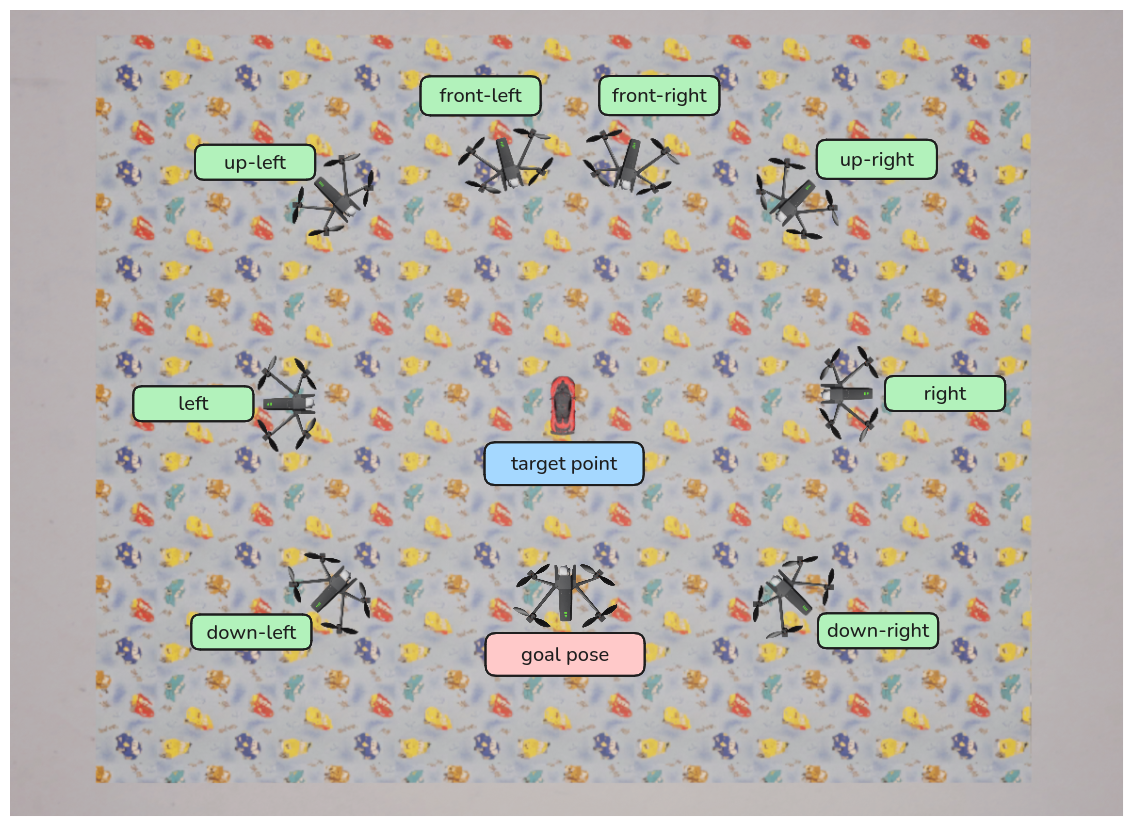
\includegraphics[width=0.8\linewidth]{Drone-Starting-Point.png}
    \caption{环境配置示意图，展示了飞行测试中目标车辆周围的 8 个起始姿态。无人机必须从每个起始姿态导航到位于车辆正后方的目标姿态，同时保持车辆始终位于相机视野内。左上、右上、左下和右下姿态相对于车辆的方位角为 $\pm45^{\circ}$，而左前和右前姿态为 $\pm14^{\circ}$。}
    \label{fig:drone-starting-poses}
\end{figure}

学生模型仅在所示每个无人机姿态上训练了 30 次仿真运行，总计 240 个训练运行样本（$74307$ 帧）。我们采用了 5 倍的数据增强（4 个增强样本 + 1 个原始样本），在每个 epoch 中通过随机饱和度变化、亮度偏移和椒盐噪声制造合成多样性，同时保留一组原始帧。数据集中的速度指令按照数据分布（表 \ref{tab:cmd-values}）在 $v_x$、$v_y$ 和 $\omega_z$ 上进行了归一化，图像则被缩放到 $224 \times 224$ 像素。由于我们的目标是输出速度指令，因此这种缩放不会影响方法性能。训练使用 Adam 优化器，学习率为 0.001，损失函数为均方误差。我们通过早停机制监控验证损失，耐心值设为 3，$\ \delta=10^{-4}$。

\begin{figure*}[!ht]
    \centering
    \begin{minipage}[t]{0.48\textwidth}
        \centering
        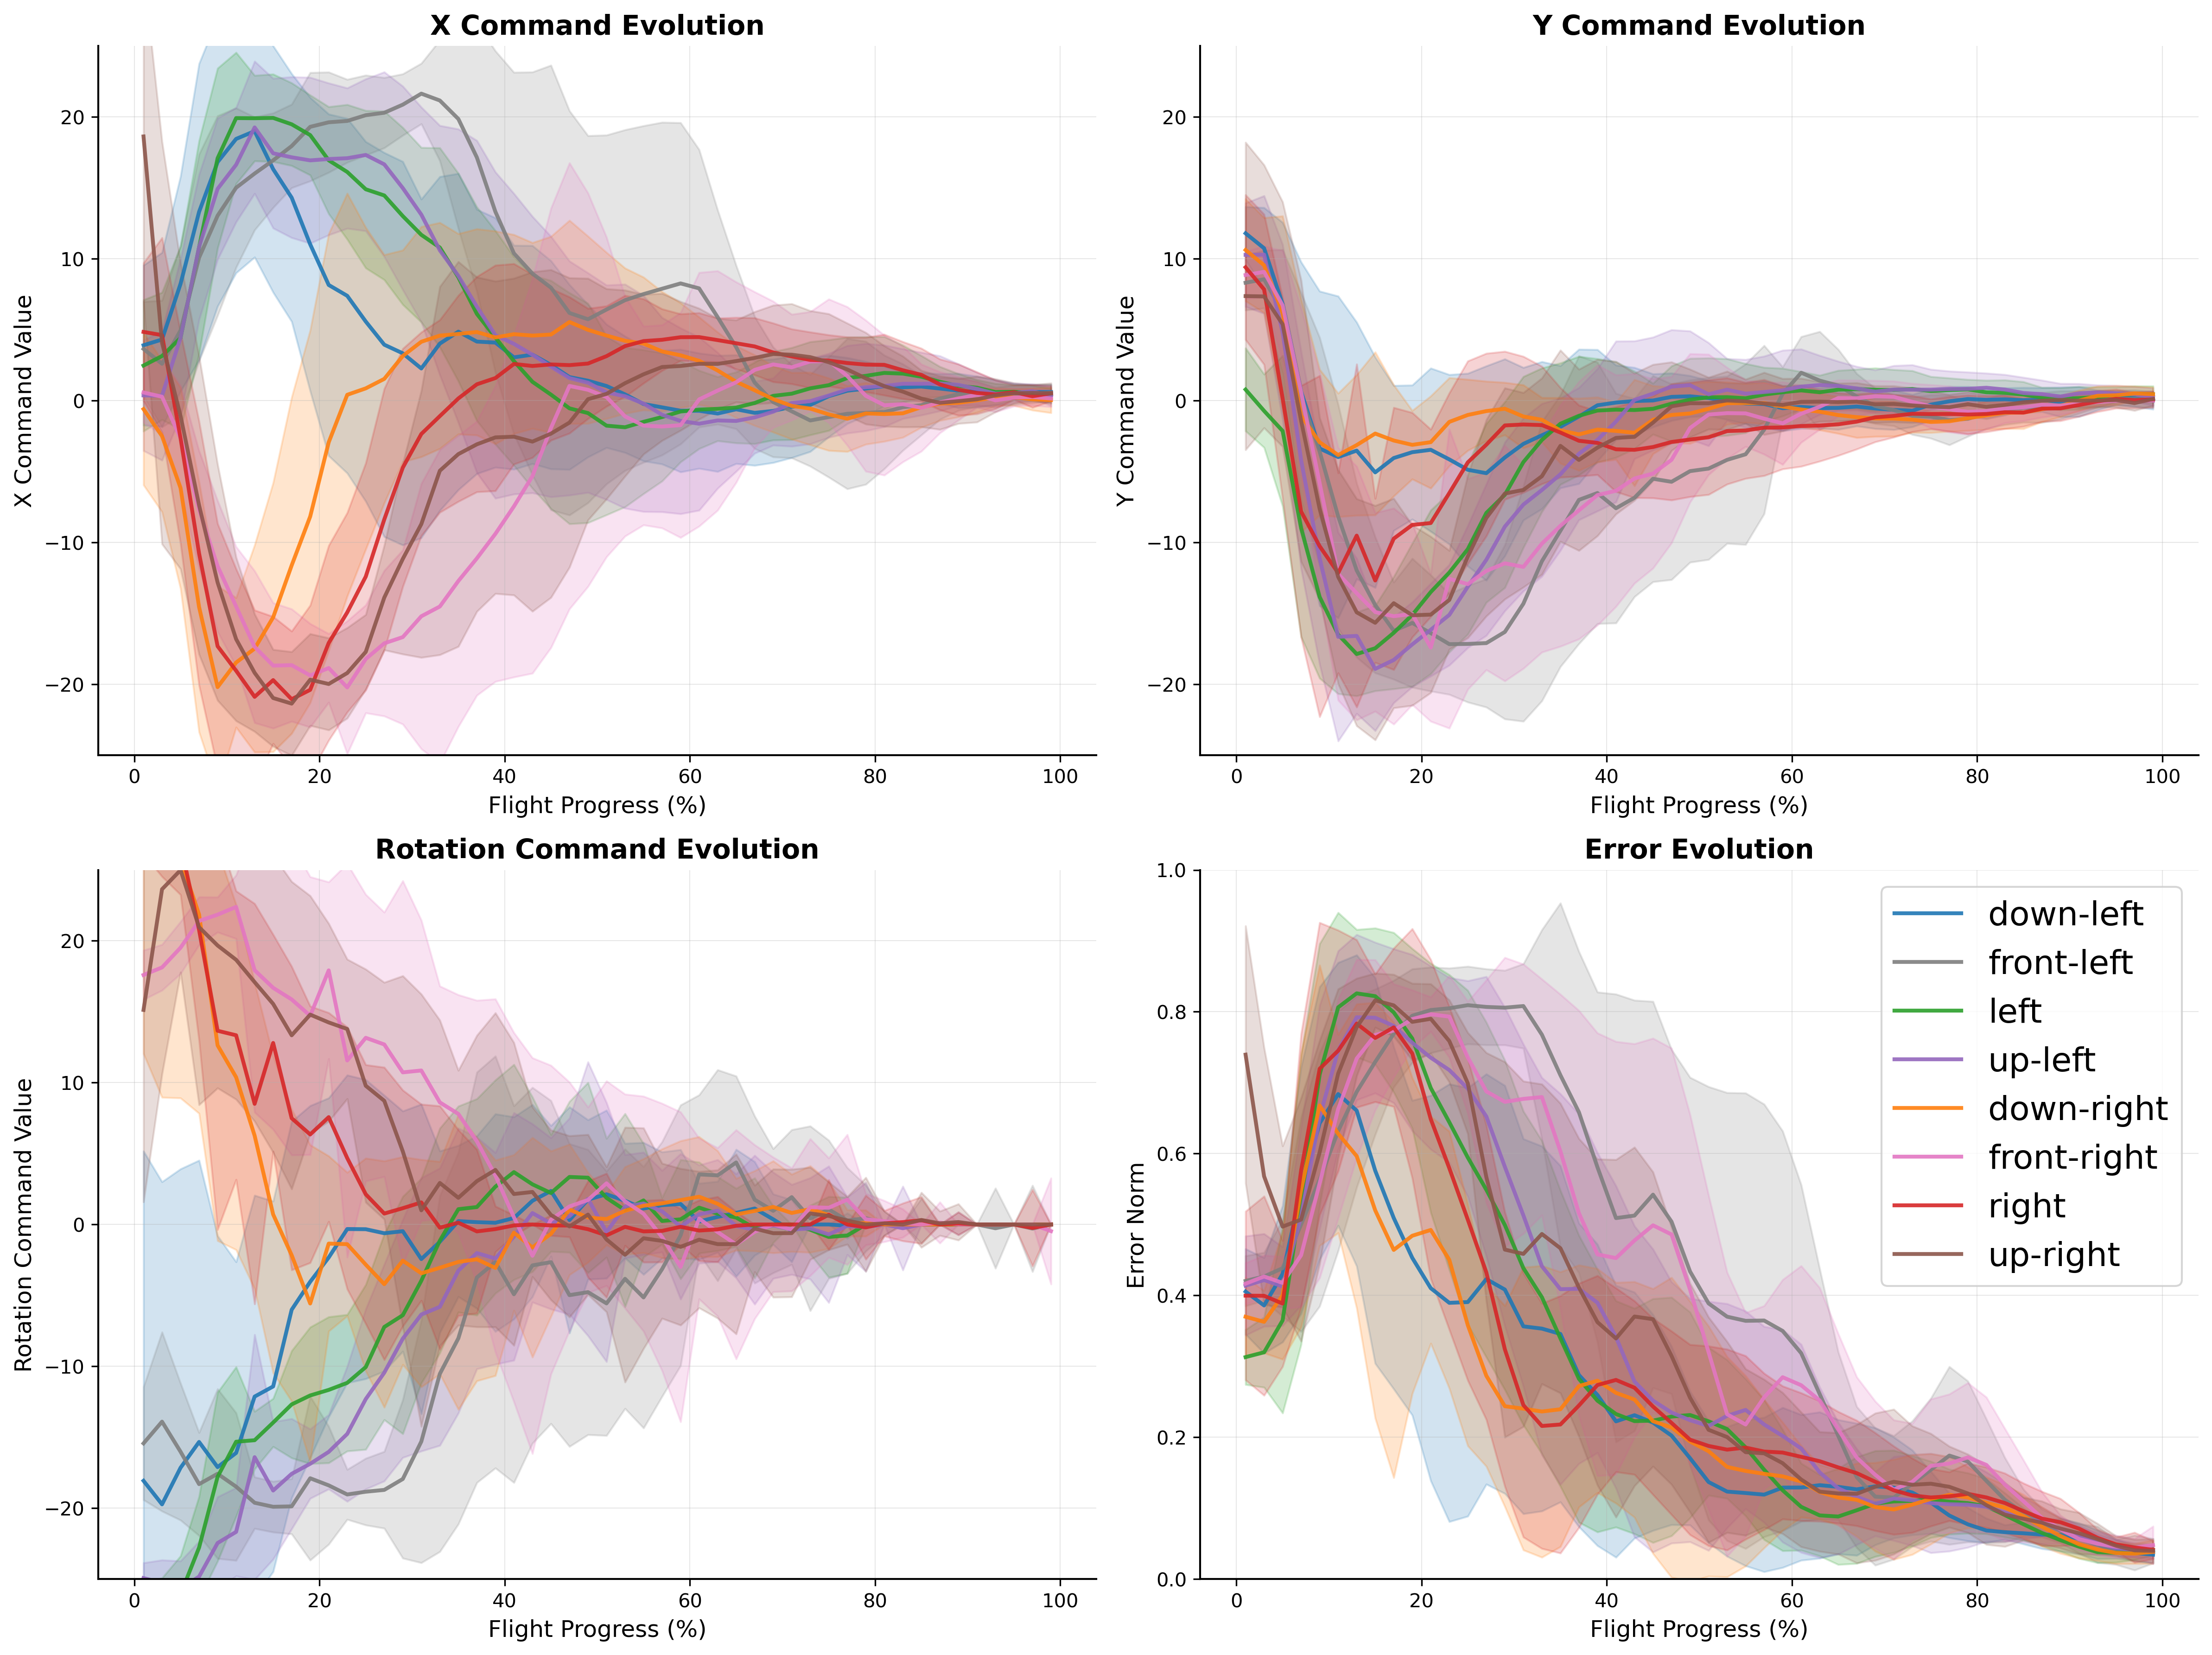
\includegraphics[width=\linewidth]{real_ibvs_evolution_over_time_commands_errors_rl_style_combined.png}
        \caption*{(a) 真实世界解析教师（NSER IBVS）：无人机控制指令和跟踪误差在飞行轨迹上的演化。}
        \label{fig:real-ibvs-evolution-over-time}
    \end{minipage}
    \hfill
    \begin{minipage}[t]{0.48\textwidth}
        \centering
        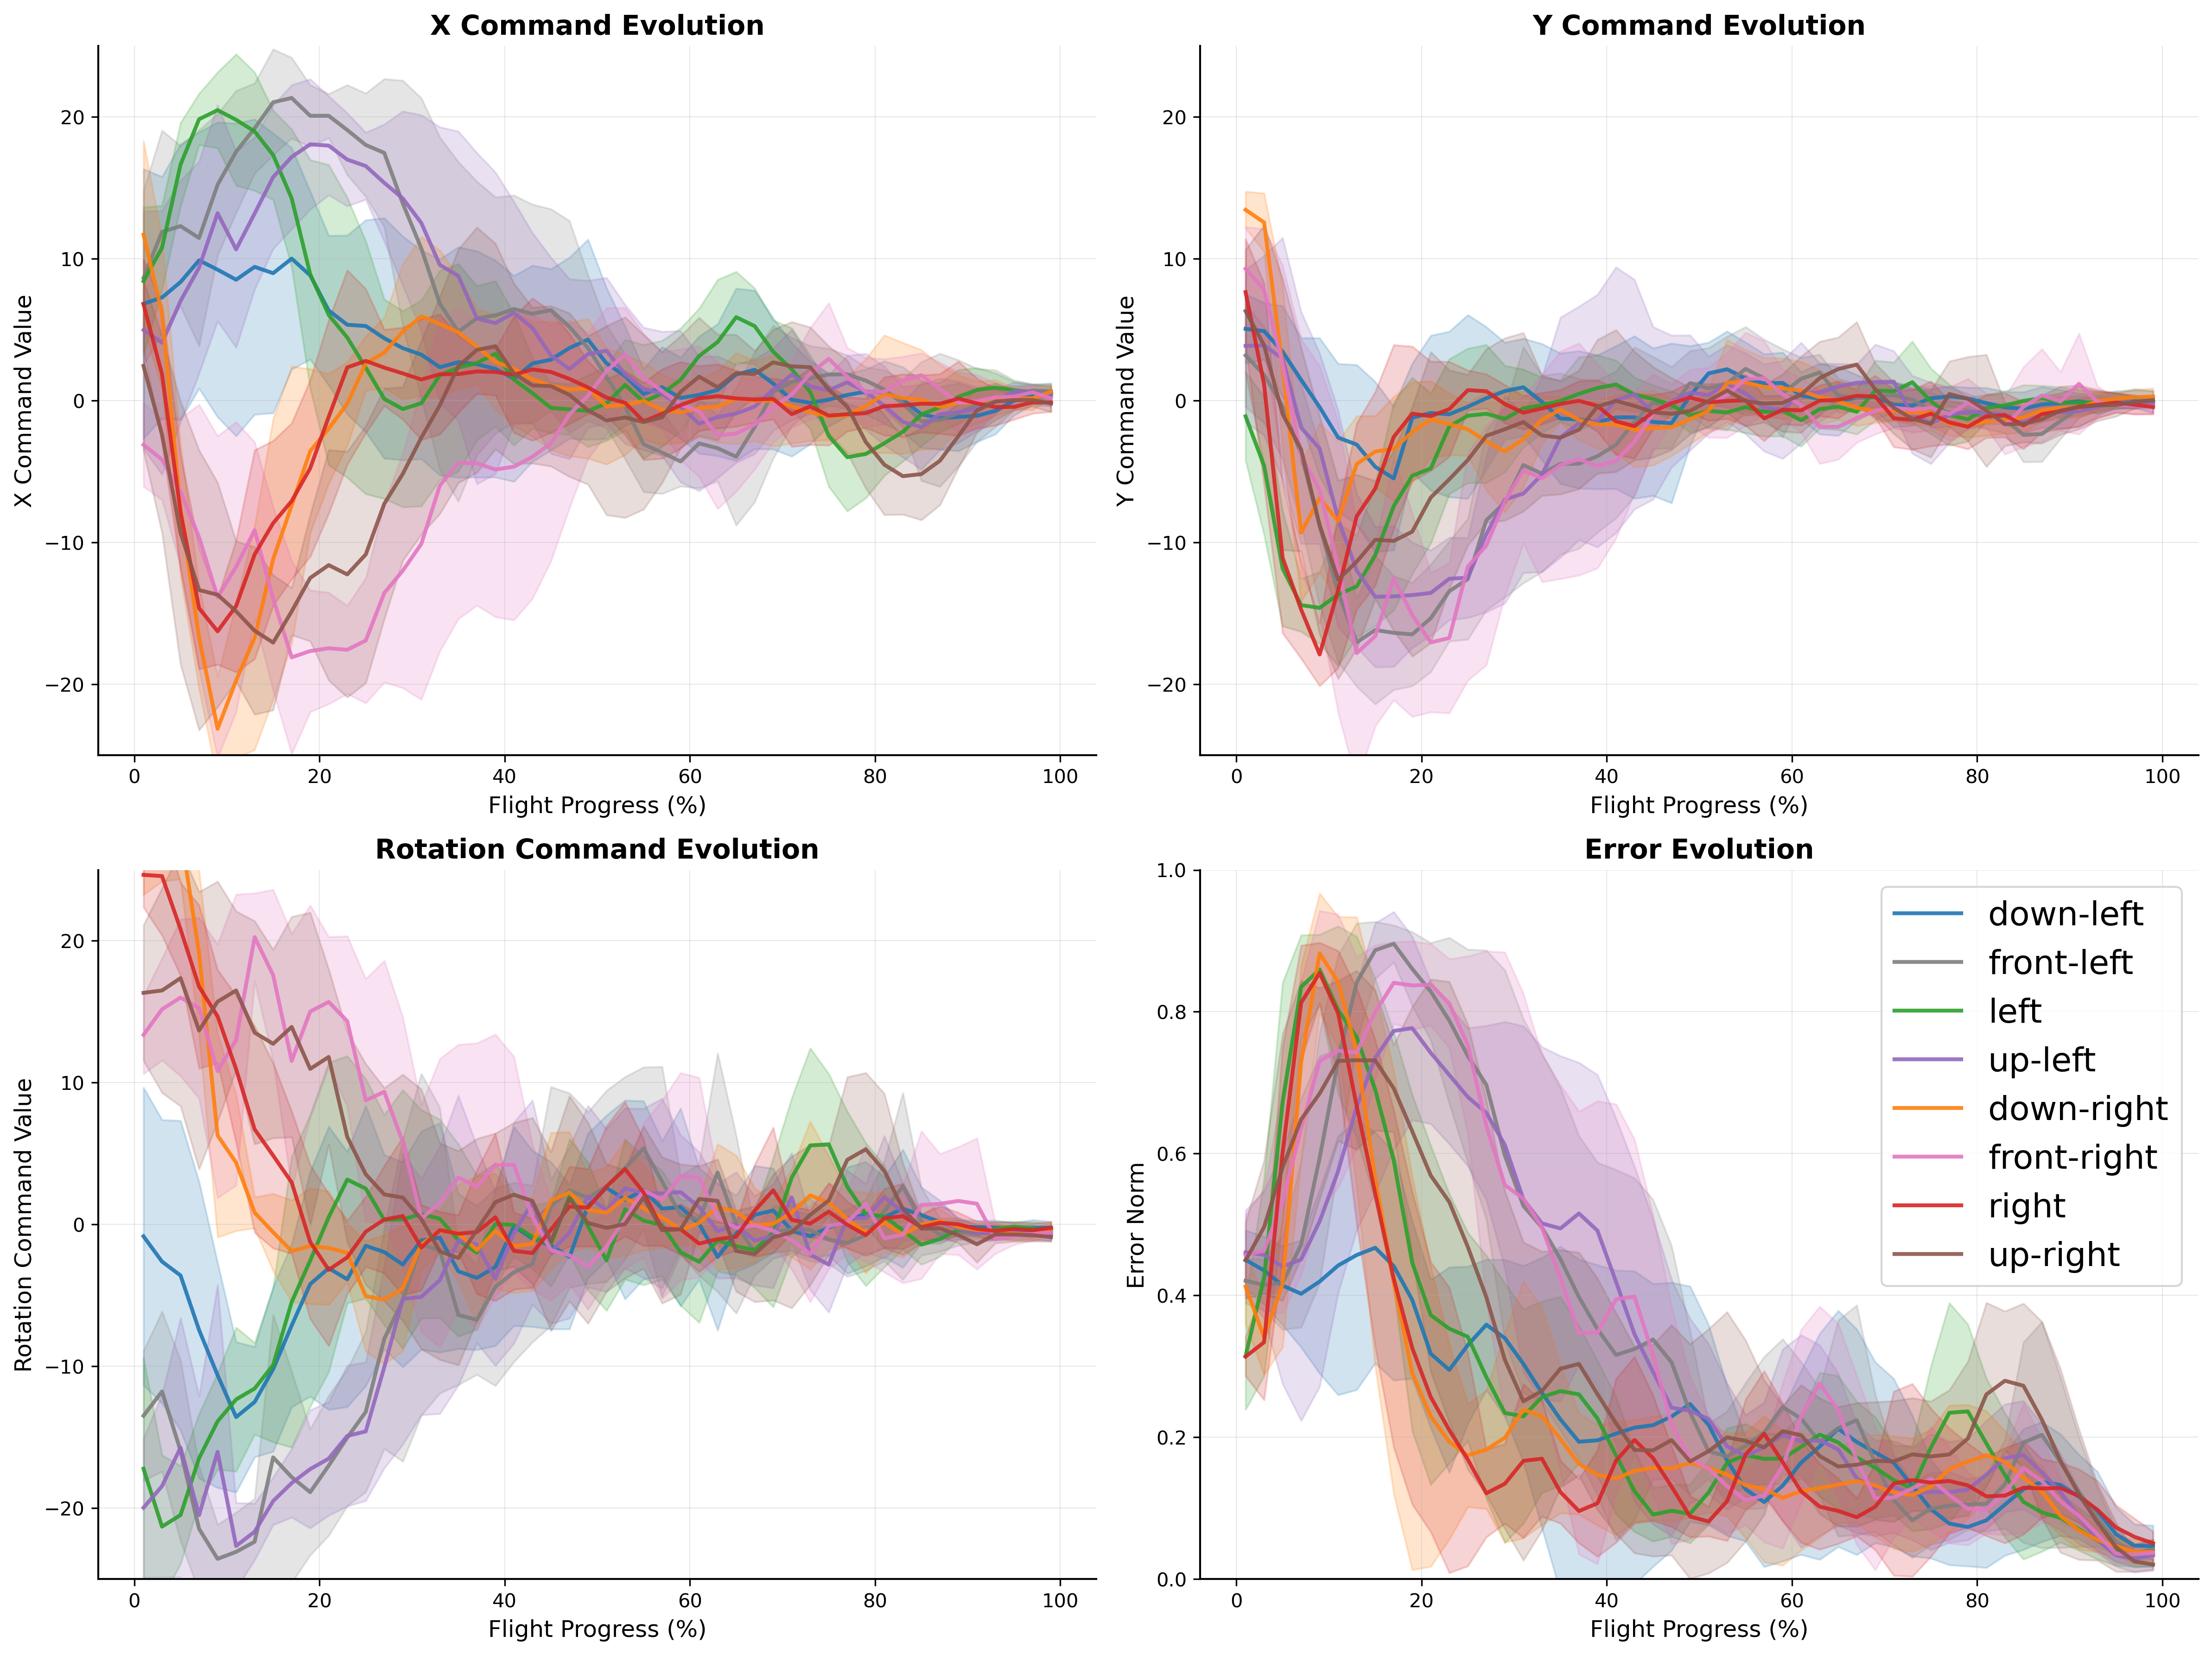
\includegraphics[width=\linewidth]{real_student_evolution_over_time_commands_errors_rl_style_combined.png}
        \caption*{(b) 真实世界小型 ConvNet 学生网络，通过蒸馏解析教师获得：无人机控制指令和跟踪误差在飞行轨迹上的演化。}
        \label{fig:real-student-evolution-over-time}
    \end{minipage}
    \caption{在来自 8 个不同起始点的飞行轨迹上，对新测试序列中 (a) 教师（NSER IBVS）和 (b) 学生（自监督神经解析）无人机控制指令与误差演化的比较（见图~\ref{fig:drone-starting-poses}）。实线表示均值；阴影区域表示不同运行之间的变化范围。所有控制指令和误差都趋于零，表明系统能够在不同初始条件下实现稳健的轨迹跟踪与控制收敛。可以看到，复杂的解析教师与小型 ConvNet 学生在无人机控制和到目标距离误差方面具有惊人的相似性。}
    \label{fig:real-evolution-comparison}
\end{figure*}

\subsection{任务终止条件}
\label{subsed:experiments-termination-conditions}
我们实现了三种终止条件，所有条件都使用尺寸为 $640 \times 360$ 像素的图像帧。首先，若无人机在 75 秒内未能校正姿态，则触发硬超时并自动降落。其次，当最近 5 个误差的中位数 $\leq 80$ 像素，且所有速度指令连续 3 秒保持为 0 时，触发软条件，这表示误差水平可接受，但可能陷入局部最优。第三，当最近 5 个误差的中位数在连续 3 秒内都 $\leq 40$ 像素时触发硬条件，这表示误差水平非常理想，此时 NSER IBVS 产生的指令很小，几乎不会引起运动。误差按包含原始像素值的向量的 L2 范数计算。

为独立评估学生模型，而不需要 IBVS 以及两个神经网络（YOLOv11 和掩码分割器），我们通过分析教师方法评估的统计结果经验性地推导出了学生终止条件。我们检查了每次评估运行最后三秒内的速度指令值。分析表明，在大多数测试中，速度指令通常位于 0 到 1 的绝对值范围内。因此，我们将其设为仿真学生的终止条件：如果最后 5 个指令的绝对值连续 3 秒都 $\leq 1$，无人机就会降落并结束测试过程。

对于真实世界环境，测试方法与仿真类似，但数据点更少。我们最初针对每个姿态测试了 10 段飞行序列，与模拟器中的设置一致（图 \ref{fig:drone-starting-poses}），共得到 80 次真实世界评估，包含 $43963$ 帧。用于真实世界部署的学生模型先在这 240 次仿真运行上预训练，再在真实世界场景上微调。真实世界中的无人机降落终止条件与仿真中完全一致。


\subsection{评估指标}
\label{subsec:experiments-metrics}
我们使用多个指标比较教师和学生模型的性能。主要指标是降落前最后三秒内图像中目标点与当前点之间的 \textbf{误差范数} 和 \textbf{交并比}（IoU）。此外，我们还测量了从跟踪开始的位置（无人机起飞且相机向下倾斜 45 度）到降落位置为止的总 \textbf{飞行时长} 和 \textbf{飞行距离}。对于学生方法，这些指标是在离线状态下计算的。

\subsection{结果与讨论}
\label{sec:discussions-results}
结果表明，与教师方法相比，学生模型获得了显著更高的跟踪精度。在仿真中，学生模型的平均误差范数为 $14.261$ 像素，而教师为 $29.756$ 像素，跟踪精度提升了 $52\%$。IoU 指标也表现出类似改进，学生为 $0.752$，教师为 $0.522$，说明目标覆盖和定位更好 \ref{tab:teacher-student-metricwise}。

\begin{table*}[htpb]
    \centering
    \small
    \setlength{\tabcolsep}{4pt}
    \renewcommand{\arraystretch}{0.9}
    \begin{tabular}{c c c c c c c c}
         &  & \multicolumn{1}{c}{\makecell{Flight SIM \\ (distance(m) / time(s)) $\downarrow$}} & \multicolumn{1}{c}{\makecell{Norm \\ Error SIM (px) $\downarrow$}} & \multicolumn{1}{c}{IoU SIM $\uparrow$} & \multicolumn{1}{c}{\makecell{Flight \\ (distance(m) / time(s)) $\downarrow$}} & \multicolumn{1}{c}{\makecell{Norm \\ Error (px) $\downarrow$}} & \multicolumn{1}{c}{IoU $\uparrow$} \\
        \addlinespace
        \cmidrule(lr){3-5} \cmidrule(lr){6-8} \multirow{2}{*}{Up-Left} & Teacher & 5.312 / \textbf{23.466} & 29.256 & 0.530 & 5.798 / \textbf{36.721} & 30.134 & 0.620 \\
                               & Student & \textbf{5.193} / 24.164 & \textbf{13.319} & \textbf{0.759} & \textbf{5.735} / 43.334 & \textbf{28.600} & \textbf{0.6263} \\
        \addlinespace
        \multirow{2}{*}{Up-Right} & Teacher & \textbf{5.675 / 24.226} & 31.800 & 0.503 & \textbf{5.622 / 41.581} & 31.499 & 0.621\\
                               & Student & 6.064 / 28.298 & \textbf{13.172} & \textbf{0.766} & 5.716 / 45.885 & \textbf{22.802} & \textbf{0.6919}\\
        \addlinespace
        \multirow{2}{*}{Front-Left} & Teacher & 6.196 / \textbf{27.315} & 30.706 & 0.517 & 6.493 / \textbf{37.535} & \textbf{28.54} & \textbf{0.611}\\
                               & Student & \textbf{6.041} / 27.917 & \textbf{13.430} & \textbf{0.758} & \textbf{6.490} / 47.238 & 33.981 & 0.560\\
        \addlinespace
        \multirow{2}{*}{Front-Right} & Teacher & \textbf{6.846 / 32.358} & 32.608 & 0.488 & \textbf{6.197 / 37.166} & 33.15 & \textbf{0.658}\\
                               & Student & 7.043 / 35.535 & \textbf{18.028} & \textbf{0.718} & 6.316 / 46.363 & \textbf{31.035} & 0.627\\
        \addlinespace
        \multirow{2}{*}{Left} & Teacher & 4.177 / \textbf{20.228} & 31.453 & 0.519 & \textbf{4.559 / 29.921} & \textbf{28.015} & 0.629\\
                               & Student & \textbf{4.089} / 20.481 & \textbf{13.243} & \textbf{0.762} & 5.065 / 43.841 & 30.853 & \textbf{0.6482} \\
        \addlinespace
        \multirow{2}{*}{Right} & Teacher & \textbf{4.317 / 19.637} & 31.137 & 0.494 & 4.831 / \textbf{41.409} & \textbf{32.423} & \textbf{0.612}\\
                               & Student & 4.518 / 21.987 & \textbf{13.798} & \textbf{0.759} & \textbf{4.811} / 57.245 & 43.672 & 0.5 \\
        \addlinespace
        \multirow{2}{*}{Down-Left} & Teacher & 2.779 / 15.988 & 28.473 & 0.518 & 4.384 / \textbf{31.622} & \textbf{28.00} & \textbf{0.611}\\
                               & Student & \textbf{2.777 / 14.900} & \textbf{13.257} & \textbf{0.763} & \textbf{4.326} / 41.044 & 39.531 & 0.5253 \\
        \addlinespace
        \multirow{2}{*}{Down-Right} & Teacher & \textbf{2.893 / 13.667} & 22.618 & 0.606 & 4.137 / \textbf{33.523} & \textbf{27.89} & \textbf{0.654}\\
                               & Student & 3.145 / 17.035 & \textbf{15.839} & \textbf{0.728} & \textbf{3.938} / 38.001 & 36.195 & 0.5478 \\
        \bottomrule
        \addlinespace
        \multirow{2}{*}{Mean} & Teacher & \textbf{4.774 / 22.111} & 29.756 & 0.522 & \textbf{5.253 / 36.185} & \textbf{29.956} & \textbf{0.627}\\
                               & Student & 4.859 / 23.790 & \textbf{14.261} & \textbf{0.752} & 5.300 / 45.369 & 33.334 & 0.591 \\
        \bottomrule
    \end{tabular}
    \caption{不同起始位置下的师生对比。左侧展示的是仿真结果；右侧展示的是现实世界飞行结果。指标包括总飞行距离/时间、最终像素范数误差（四个角点组合后的误差向量的 L2 范数）以及最终 IoU（L2 范数和 IOU 均在飞行最后 3 秒内计算）。教师的飞行时间略快。然而，学生的计算速度快了 $11\times$（见表 \ref{tab:nn-timing-eval}）。在训练更多的仿真场景中，学生在精度上略优于教师（到达目标时误差更低）；但在仅用较少飞行数据训练的真实世界场景中，学生的精度略低。}
    \label{tab:teacher-student-metricwise}
\end{table*}

轨迹演化分析表明，两种方法都能成功收敛到目标，但其特征不同。教师方法的指令更为保守、收敛更渐进，而学生方法则表现出更直接的路径和更快的误差下降速率，如图 \ref{fig:trajectory-ibvs} 所示。

\begin{figure}
    \centering
    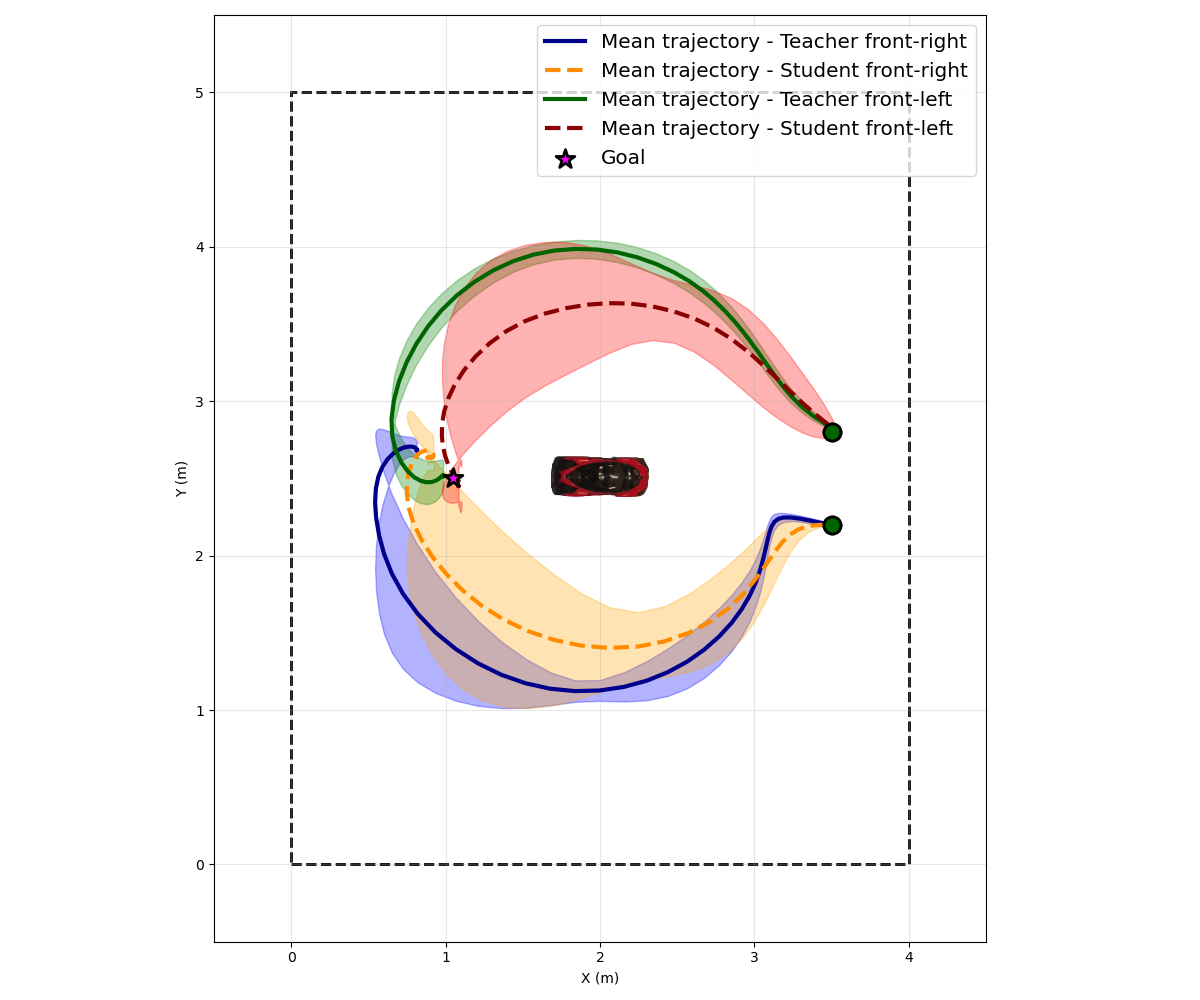
\includegraphics[width=\linewidth]{trajectories_sim_teacher_student_front.png}
    \caption{教师和学生仿真飞行轨迹的对比，展示了两个起始姿态（绿色圆圈：左前和右前）的均值与标准差。实线蓝色和绿色曲线表示教师 NSER IBVS 方法的平均路径，而虚线橙色和红色曲线表示学生路径。阴影区域表示不同运行之间的轨迹变化。星号表示目标姿态。可以注意到，学生路径的变化更大，但其平均路径比教师更短。}
    \label{fig:trajectory-ibvs}
\end{figure}

为比较我们提出的学生网络在有无分割情况下与基线 NSER IBVS 的计算效率，我们在一组分辨率为 $640 \times 360$ 的真实世界帧上进行了运行时间基准测试。每个评估器都独立处理相同的输入帧集，我们在 30 次重复试验中测量了逐帧推理时间，以考虑系统负载和内存影响带来的波动。每次试验前，我们都进行了预热迭代以避免初始化偏差，并在各次运行之间显式释放内存。我们将推理时间以毫秒和 FPS 形式报告。结果汇总见表 \ref{tab:nn-timing-eval}。 

\begin{table}[t]
\centering
\footnotesize
\caption{30 次试验中的计算时间（毫秒）。这个 1.7M 参数的小型学生 ConvNet 比教师快 $11\times$。}
\label{tab:nn-timing-eval}
\begin{tabular}{lrrrrrr}
\toprule
\textbf{Evaluator} & \textbf{Avg} & \textbf{Std} & \textbf{Med} & \textbf{Min} & \textbf{Max} & \textbf{FPS} \\
\midrule
NSER IBVS & 20.69 & 7.63 & 24.56 & 6.45 & 82.55 & 48.30 \\
Student  & \textbf{1.85} & 0.93 & 1.84 & 1.79 & 235.64 & \textbf{540.8} \\
\bottomrule
\end{tabular}
\end{table}

结果表明，仿真到现实的迁移是有效的，尽管如预期那样存在一定性能下降。在真实世界场景中，学生模型保持了有竞争力的跟踪精度，而教师方法在不同环境下表现更稳定。使用 80 个真实世界场景进行微调的方法在领域自适应方面是有效的，使其能够成功部署到实际场景中。

\section{总结与结论}
\label{sec:conclusion}
本文通过高效知识蒸馏提出了首个用于无人机视觉伺服的自监督神经解析系统：一个小型 ConvNet 学生从所提出的、数值稳定的解析教师（NSER-IBVS）中学习，使无人机能够从不同起始姿态飞行到目标姿态，并完整覆盖三角圆上的相对姿态差异。该系统完全无监督，不需要任何人工干预、监督式预训练或外部传感器，这与文献中的其他方法不同。该学生网络只有 1.7M 参数，易于部署到嵌入式设备上，其计算速度比教师路径快 $11\times$（$529.77$ FPS 对比 $48.3$ FPS），同时在仿真和真实世界测试中都保持了同样的飞行精度和速度。真实世界案例的学习仅限于少量飞行（$80$ 次），以进一步降低成本，这得益于在数字孪生仿真环境与真实场景之间的高效迁移。

我们提出的新型两阶段分割流水线将 YOLOv11 与专用的基于 U-Net 的掩码分割器结合起来，在不需要显式几何模型或人工标记的情况下，实现了稳健的车辆前后区域分割。该方法的自监督特性已通过仿真到现实的迁移学习以及在 Parrot Anafi 无人机平台上的测试得到验证，证明了其在硬件基础设施要求极低的情况下实现完全自主室内运行的实际可行性。 

针对完全覆盖三角圆的不同无人机姿态所做的实验验证证实了我们无监督方法的有效性。虽然与教师相比，学生网络在真实世界中的像素误差略高（由于真实训练飞行非常有限，平均误差为 $29.956$ 对 $33.334$ 像素），但它仍保持了可接受的 IoU 性能（$0.627$ 对 $0.591$），并实现了更快的收敛时间。值得注意的是，在进行更充分自监督训练的仿真环境中，系统表现出更优的收敛时间和更低的误差，验证了基于仿真的训练相较于昂贵的真实世界数据采集更具成本效益。计算效率的提升使我们的方法尤其适用于资源受限平台上的实时应用，并为无需人工监督或标记依赖的自主视觉伺服建立了新的范式。

\section*{致谢} 
本工作部分得到以下项目支持：“Romanian Hub for Artificial Intelligence - HRIA”、Smart Growth、Digitization and Financial Instruments Program, 2021-2027（MySMIS 编号 334906）、European Health and Digital Executive Agency（HADEA）在欧盟委员会授权下通过 DIGITWIN4CIUE 项目提供的资助（协议号 101084054），以及“European Lighthouse of AI for Sustainability - ELIAS”、Horizon Europe 计划（资助号 101120237）。
{
\small
\bibliographystyle{ieeenat_fullname}
\bibliography{main}
}

\end{document}
\typeout{get arXiv to do 4 passes: Label(s) may have changed. Rerun}
